\documentclass[10pt]{article}
\usepackage{icmlko}

\icmlmeta{IP 파운데이션 월드모델}{184}{셋 다 같은 답을 주는데 하나만 가른다}{노트 183이 ``판이 크기 가중이라 작은 도메인을 숨긴다''를 남겼다. 가중을 셋으로 바꿔 열 형태를 다시 채점했다 --- 순위는 안 바뀌고 분해능이 바뀐다}

\begin{document}

\twocolumn[
\icmlheader

\begin{abstract}
노트 183이 ``팝업이 반 토막 나도 판은 0.005 내려간다''를 보이고 ``최소
도메인 $\rho$ 를 나란히 적을 것인가''를 남겼다. 답하려면 재야 한다 ---
열 형태를 \textbf{크기 가중 · 도메인 균등 · 최소 도메인} 세 기준으로 다시
채점했다. \textbf{순위는 거의 안 바뀐다} --- 크기 대 균등의 순위 상관이
$\rho{=}\mathbf{+0.964}$ 이고 크기 대 최소가 $+$0.709 다. \textbf{F18
배깅이 세 기준 모두에서 1위}이고(최소 기준에서 F8 이 점수로 $+$0.003
앞서지만 짝 검정에서 F18 이 62\% 이긴다 --- 못 가른다) 꼴찌들도 그대로다.
\textbf{그런데 분해능이 완전히 다르다.} F18 이 다른 넷을 이길 붓스트랩
확률은 크기 가중에서 \textbf{네 번 다 100\%}($t{=}2.3{\sim}5.9$), 도메인
균등에서 86$\sim$99\%($t{=}1.1{\sim}2.4$), \textbf{최소 도메인에서
62$\sim$72\%}($t{=}0.3{\sim}0.6$)다. \textbf{최소 도메인 기준은 다섯
형태 중 어느 둘도 못 가른다} --- 오차막대가 $\pm$0.13 이다. 최소가 대개
표본 스물다섯짜리 아이돌이나 여든짜리 펀딩이라 그렇다. \textbf{그러니
노트 82 · 90 의 크기 가중 선택이 근거를 하나 새로 얻는다} --- 편해서가
아니라 \emph{가를 수 있는 유일한 가중}이라서다. 곁가지로 둘. ① 챔피언은
넓게 이긴다 --- F18 이 F6 능형을 \textbf{아홉 도메인 중 여덟}에서 이기고
(가중 97.7\%) 지는 하나가 \textbf{팝업}($-$0.070)이다. 중앙값 기준에서
F9 · F6 이 F18 을 앞서는 것처럼 보이는데, 정렬해 보면 F18 이 아홉 자리 중
여덟에서 위다 --- \textbf{중앙값 역전은 순서 통계량의 우연이다.}
② 우연 판($F0$)이 크기 가중에서 $+$0.0126 이고 균등에서 $-$0.0127 인데
\textbf{둘 다 0 에서 0.6 · 0.4 sd 로 잡음 안}이다.
\end{abstract}
]

\begin{figure*}[t]
\centering
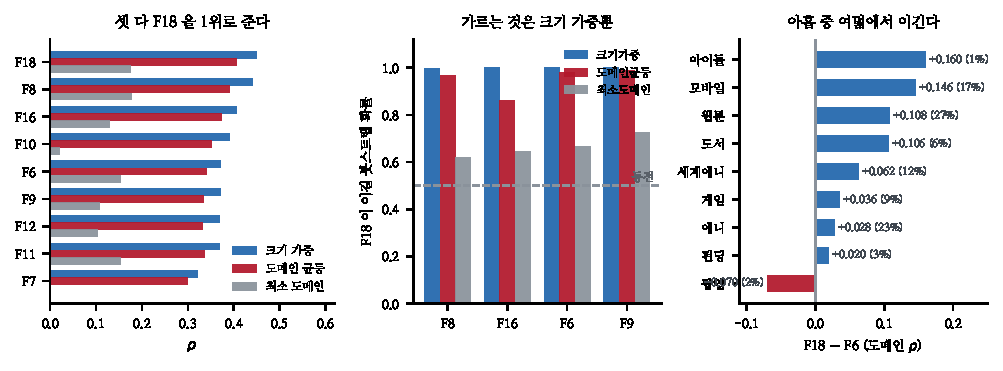
\includegraphics[width=\textwidth]{figs/weight.pdf}
\caption{왼쪽 --- 셋 다 F18 을 1위로 준다. 가운데 --- 가르는 것은 크기
가중뿐. 오른쪽 --- 아홉 중 여덟에서 이긴다.}
\end{figure*}

\section{순위는 안 바뀐다}

\begin{table}[t]
\centering\tsize
\caption{세 기준. 유보 2,608건 · 아홉 도메인.}
\begin{tabular}{lrrr}
\toprule
& 크기 가중 & 도메인 균등 & 최소 도메인 \\
\midrule
\textbf{F18 배깅} & \textbf{.4490} & \textbf{.4062} & .1753 \\
F8 부스트 & .4404 & .3905 & \textbf{.1783} \\
F16 몸통머리 & .4060 & .3738 & .1289 \\
F6 능형 & .3709 & .3399 & .1536 \\
F9 순위가능도 & .3705 & .3340 & .1084 \\
F10 도메인축소 & .3914 & .3521 & .0212 \\
F7 앵커 & .3206 & .2990 & $-$.0123 \\
\midrule
F0 우연 & $+$.0126 & $-$.0127 & $-$.0819 \\
\bottomrule
\end{tabular}
\end{table}

\claimx{\textbf{크기 대 균등의 순위 상관이 $+$0.964 다.} F18 이 셋 다
1위이고 F7 앵커가 셋 다 꼴찌다. \textbf{가중을 바꿔도 챔피언이 안
바뀐다.}}{노트 183이 걱정한 것은 실재하지만 \emph{순위}에는 안 나타난다
--- 작은 도메인이 숨겨지는 것은 \emph{변화를 진단할 때} 문제이지 형태를
줄 세울 때 문제가 아니다.}

\claimx{\textbf{우연 판이 크기에서 $+$0.0126 이고 균등에서 $-$0.0127
이다.} 부호가 반대라 놀라 보이지만 표준오차가 각각 0.0196 · 0.031 이라
\textbf{둘 다 0 에서 0.6 · 0.4 sd} 다.}{큰 도메인 넷이 다 작은 양수이고
작은 도메인 다섯이 다 음수인 것이 그 차이를 만든다. \textbf{아홉 개로는
그런 갈림이 우연히 나온다.}}

\section{분해능이 다르다}

\begin{table}[t]
\centering\tsize
\caption{F18 이 이길 붓스트랩 확률. 짝 400회.}
\begin{tabular}{lrrr}
\toprule
& 크기 & 균등 & 최소 \\
\midrule
vs F8 부스트 & \textbf{100\%} & 97\% & \textbf{62\%} \\
vs F16 몸통머리 & \textbf{100\%} & 86\% & 65\% \\
vs F6 능형 & \textbf{100\%} & 98\% & 66\% \\
vs F9 순위가능도 & \textbf{100\%} & 99\% & 72\% \\
\midrule
$t$ 범위 & 2.3$\sim$5.9 & 1.1$\sim$2.4 & \textbf{0.3$\sim$0.6} \\
\bottomrule
\end{tabular}
\end{table}

\claimx{\textbf{최소 도메인 기준은 아무것도 못 가른다.} 다섯 형태 어느
쌍도 $t{<}0.6$ 이고 이길 확률이 동전에 가깝다. 짝 sd 가
\textbf{$\pm$0.13} 이다.}{까닭이 뻔하다 --- 최소가 대개 표본 스물다섯짜리
아이돌이거나 여든짜리 펀딩이다. 노트 152의 검출 한계로 그 표본의 짝
반폭이 0.2 를 넘는다. \textbf{최소는 정의상 제일 시끄러운 도메인을 고른다.}}

\claimx{\textbf{그래서 노트 82 · 90 의 선택이 근거를 새로 얻는다.} 크기
가중을 고른 것은 편해서가 아니라 \textbf{가를 수 있는 유일한 가중}이라서다
--- 균등도 되지만 $t$ 가 절반이고, 최소는 안 된다.}{이건 원래 근거와
다르다. 노트 82 는 ``작은 도메인의 $\rho$ 는 오차가 커서 같은 무게를 주면
잡음이 순위를 흔든다''고 적었는데, \textbf{여기서는 그 예측이 실제로
확인됐다} --- 균등에서 $t$ 가 절반으로 준다.}

\section{챔피언은 넓게 이긴다}

\begin{table}[t]
\centering\tsize
\caption{F18 배깅 $-$ F6 능형. 도메인별.}
\begin{tabular}{lrrr}
\toprule
& 몫 & 차 & \\
\midrule
아이돌 & 1.0\% & $+$.160 & \\
모바일 & 16.9\% & $+$.146 & \\
웹툰 & 27.3\% & $+$.108 & \\
도서 & 6.2\% & $+$.107 & \\
세계애니 & 11.5\% & $+$.062 & \\
게임 & 8.6\% & $+$.036 & \\
애니 & 23.2\% & $+$.028 & \\
펀딩 & 3.1\% & $+$.020 & \\
\midrule
\textbf{팝업} & \textbf{2.3\%} & \textbf{$-$.070} & 유일한 패배 \\
\bottomrule
\end{tabular}
\end{table}

\claimx{\textbf{아홉 중 여덟, 가중 97.7\%에서 이긴다.} 챔피언의 우위가
큰 도메인에만 있는 것이 아니다 --- 아이돌(1.0\%)에서 $+$0.160 으로 제일
크게 이긴다.}{\textbf{지는 하나가 팝업이다.} 노트 183이 ``출발점이
사라지고 있다''로 닫은 그 도메인에서, 챔피언이 능형보다 못하다.}

\claimx{\textbf{중앙값 역전은 순서 통계량의 우연이다.} 중앙 도메인
$\rho$ 로는 F9($+$.4166) · F6($+$.4124)이 F18($+$.4023)을 앞선다. 그런데
아홉 값을 정렬해 견주면 \textbf{F18 이 아홉 자리 중 여덟에서 위}이고
다섯째 자리에서만 아래다.}{\textbf{이걸 안 갈랐으면 ``선형이 보통
도메인에서 낫다''로 적을 뻔했다} --- 노트 155부터 여덟 번 확인한 나무 대
선형 이야기에 딱 맞는 모양이라 더 위험했다. \textbf{맞는 이야기에 맞는
모양의 잡음이 제일 위험하다.}}

\begin{table}[t]
\centering\tsize
\caption{남은 것.}
\begin{tabular}{ll}
\toprule
\textbf{팝업} & 챔피언이 능형에 지는 유일한 도메인 \\
균등 가중 & $t$ 가 절반 --- 나란히 적을 값은 있나 \\
F8 & 최소 도메인에서만 F18 을 앞선다(못 가름) \\
\bottomrule
\end{tabular}
\end{table}

첫 줄이 다음이다. F18 배깅이 팝업에서 $+$0.343 이고 F6 능형이 $+$0.412 다
--- 아홉 도메인 중 유일하게 뒤집힌다. 팝업은 유보 59건이라 짝 반폭이
0.124(노트 152)이므로 이 0.070 차이는 안 갈린다. \textbf{그래도 방향이
일관되면 뜻이 있다} --- 팝업 축 다섯이 전부 사람이 읽어 매긴 것이고
(노트 154 · 173), 사람이 매긴 축은 잡음이 적고 선형에 가까울 수 있다.
\textbf{그러면 ``사람이 매긴 축에서는 선형이 낫다''가 되고, 그건 손잡이
쪽에서 큰 이야기다.}

\end{document}
